% Copyright 2005-2016 Airbus-EDF-IMACS-Phimeca
% Permission is granted to copy, distribute and/or modify this document
% under the terms of the GNU Free Documentation License, Version 1.2
% or any later version published by the Free Software Foundation;
% with no Invariant Sections, no Front-Cover Texts, and no Back-Cover
% Texts.  A copy of the license is included in the section entitled "GNU
% Free Documentation License".
\renewcommand{\nomfichier}{docref_C311_TransIso_GeneralizedNataf}
\renewcommand{\titrefiche}{Generalized Nataf Transformation}

\Header

\MathematicalDescription{
  \underline{\textbf{Goal}} \vspace{2mm}

  The Generalized Nataf transformation is an isoprobabilistic transformation (refer to \otref{docref_C311_TransIso}{Isoprobabilistic Transformation}) which is used under the following context : $\vect{X}$ is the input random vector,  $F_i$ the cumulative density functions of its components and $C$ its copula, which is supposed to be elliptical.\\

  Let us denote by $\vect{d}$ a determinist vector, $g(\vect{X}\,,\,\vect{d})$ the limit state function of the model, $\cD_f = \{\vect{X} \in \Rset^n \, / \, g(\vect{X}\,,\,\vect{d}) \le 0\}$ the  event considered here and {g(\vect{X}\,,\,\vect{d}) = 0} its boundary.\\

  One way to evaluate the probability content of the event $\cD_f$:
  \begin{equation}\label{PfX}
    P_f = \Prob{g(\vect{X}\,,\,\vect{d})\leq 0}=   \int_{\cD_f}  \pdf\, d\vect{x}
  \end{equation}
  is to use the Generalized Nataf transformation  $T$  which is a diffeomorphism from $\supp(\vect{X})$ into the standard space $\Rset^n$, where distributions are spherical, with zero mean, unit variance and unit correlation matrix. The type of the spherical distribution is the type of the elliptical copula $C$.

  The Generalized Nataf transformation presented here is a generalisation of the traditional Nataf transformation (see [A. Nataf]) : the reference [R. Lebrun, A. Dutfoy a] shows that the Nataf transformation can be used only if the copula of $\vect{X}$ is normal. The Generalized Nataf transformation (see [R. Lebrun, A. Dutfoy b]) extends the Nataf transformation to elliptical copulas.

  \vspace{2mm}

  \underline{\textbf{Principle}} \vspace{2mm}

  Let us recall some definitions.\\

  A random vector $\vect{X}$ in $\Rset^n$ has an \emph{elliptical distribution} if and only if there exists a deterministic vector $\vect{\mu}$ such that the characteristic function of $\vect{X} - \vect{\mu}$ is a scalar function of the quadratic form $\vect{u}^t\mat{\Sigma}\, \vect{u}$:
  \begin{align*}
    \varphi_{\vect{X}-\vect{\mu}}(\vect{u})=\psi(\vect{u}^t\,\mat{\Sigma}\, \vect{u})
  \end{align*}
  with $\mat{\Sigma}$ a symmetric positive definite matrix of rank $p$. As $\mat{\Sigma}$ is symmetric positive, it can be written in the form $\mat{\Sigma}=\mat{D}\,\mat{R}\,\mat{D}$, where $\mat{D}$ is the diagonal matrix $\mat{\diag{\sigma_i}}$ with $\sigma_i=\sqrt{\Sigma_{ii}}$ and $R_{ij}=\frac{\Sigma_{ij}}{\sqrt{\Sigma_{ii}\Sigma_{jj}}}$.\\
  With a specific choice of normalisation for $\psi$, in the case of finite second moment, the covariance matrix of $\vect{X}$ is $\mat{\Sigma}$ and $\mat{R}$ is then its linear correlation matrix. The matrix $\mat{R}$ is always well-defined, even if the distribution has no finite second moment: even in this case, we call it the correlation matrix of the distribution. We note $\vect{\sigma}=(\sigma_1,\dots,\sigma_n)$.\\

  We denote by $E_{\vect{\mu},\vect{\sigma},\mat{R},\psi}$ the cumulative distribution function of the elliptical distribution $\cE_{\vect{\mu},\vect{\sigma}, \mat{R},\psi}$.\\

  An \emph{elliptical copula} $C^E_{\mat{R},\psi}$ is the copula of an elliptical distribution $\cE_{\vect{\mu},\vect{\sigma},\mat{R},\psi}$.\\

  The \emph{generic elliptical representative} of an elliptical distribution family $\cE_{\vect{\mu},\vect{\sigma},\mat{R},\psi}$ is the elliptical distribution whose cumulative distribution function is $E_{\vect{0},\vect{1},\mat{R},\psi}$.\\

  The \emph{standard spherical representative} of an elliptical distribution family $\cE_{\vect{\mu},\vect{\sigma},\mat{R},\psi}$ is the spherical distribution whose cumulative distribution function is $E_{\vect{0},\vect{1},\mat{I}_n,\psi}$.\\

  The family of distributions with marginal cumulative distribution functions are $F_1,\dots,F_n$ and any elliptical copula $C^E_{\mat{R},\psi}$ is denoted by ${\cD}_{F_1,\dots,F_n,C^E_{\mat{R},\psi}}$. The cumulative distribution function of this distribution is noted $D_{F_1,\dots,F_n,C^E_{\mat{R},\psi}}$.\\

  The random vector $\vect{X}$ is supposed to be continuous and with full rank. It is also supposed that its cumulative marginal distribution functions $F_i$  are strictly increasing (so they are bijective) and that the matrix $\mat{R}$ of its elliptical copula is symmetric positive definite.\\

  {\bf Generalized Nataf transformation}:   Let $\vect{X}$ in $\Rset^n$ be a continuous random vector following the distribution $D_{F_1,\dots,F_n,C^E_{\mat{R},\psi}}$. The \emph{Generalized Nataf transformation} $T_{Nataf}^{gen}$ is defined by:
  \begin{equation}
    \vect{u} = T_{Nataf}^{gen}(\vect{X})=T_3\circ T_2\circ T_1(\vect{X})
  \end{equation}
  where the three transformations $T_1$, $T_2$ and $T_3$ are given by:
  \begin{equation}
    \begin{array}{l}
      \begin{array}{rcl}
        T_1 : \Rset^n & \rightarrow & \Rset^n\\
        \vect{x} & \mapsto & \vect{w}=\Tr{(F_1(x_1),\dots,F_n(x_n))}
      \end{array}\\
      \begin{array}{rcl}
        T_2 : \Rset^n & \rightarrow & \Rset^n\\
        \vect{w} & \mapsto & \vect{v}=\Tr{(E^{-1}(w_1),\dots,E^{-1}(w_n))}
      \end{array}\\
      \begin{array}{rcl}
        T_3 : \Rset^n & \rightarrow & \Rset^n\\
        \vect{v} & \mapsto & \vect{u}=\mat{\Gamma}\,\vect{v}
      \end{array}
    \end{array}
  \end{equation}
  where $E$ is the cumulative distribution function of the standard 1-dimensional elliptical distribution with characteristic generator $\psi$ and $\mat{\Gamma}$ is the inverse of the Cholesky factor of $\mat{R}$.\\

  The distribution of $\vect{W}=T_2\circ T_1(\vect{X})$ is the generic elliptical representative associated to the copula of $\vect{X}$. The step $T_3$ maps this distribution into its standard representative, following exactly the same algebra as the normal copula. Thus, in the Generalized Nataf standard space, the random vector $\vect{U}$ follows the standard representative distribution of the copula of the physical random vector $\vect{X}$. \\
  If the copula of $\vect{X}$ is normal,  $\vect{U}$ follows the standard normal distribution with independent components.


  % \begin{figure}[Hhtbp]
  \begin{center}\label{genNataf}
    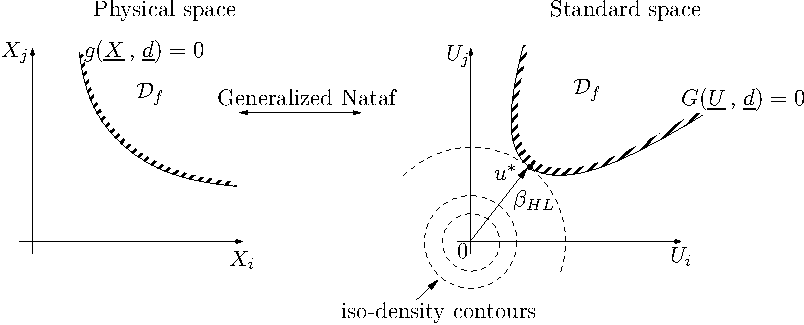
\includegraphics{Figures/FigureNatafGener.pdf}
    % \caption{ }
  \end{center}
  % \end{figure}


}
{
  --}

\Methodology{
  Within the global methodology, the isoprobabilistic transformation is used in the First and Second Order reliability Method to evaluate  the probability content of the event $\cD_f$ (refer to \otref{docref_C311_Form}{FORM} and \otref{docref_C311_Sorm}{SORM}). It is an alternative to the Rosenblatt  transformation (refer to \otref{docref_C311_TransIso_Rosenblatt}{Rosenblatt}) in the case where the copula is  elliptical (refer to \otref{docref_C311_TransIso}{Isoprobabilistic Transformation} for more details on isoprobabilistic transformations).\\
  OpenTURNS uses the Generalized Nataf transformation to map in the standard space any random vector which copula is elliptical.
}
            {

              Traditionnally, the Nataf transformation is used in the case where the information on the random vector $\vect{X}$ is limited to the distributions of its components $F_i$ and its linear correlation matrix  (or Pearson correlation coefficient, refer to \otref{docref_B231_Pearson}{Pearson correlation coefficient}). It is important to note that the Nataf transformation adds some information on the dependence structure by modeling it with a normal copula. This \emph{implicit hypothesis} might have a great impact on the precision of the evaluation of the event probability (see [R. Lebrun, A. Dutfoy, 2008, a]). That's why the Nataf transformation may be used only if it has been verified whether the normal copula is a proper modelisation of the dependence structure of the random vector $\vect{X}$. \\

              Furthermore, the normal copula of the random vector $\vect{X}$ is parameterized from its linear correlation matrix, which arises some problems due to the fact that the linear correlation matrix is not a usefull indicator of the dependence between two correlated variables (see [R. Lebrun, A. Dutfoy, 2008, a]). More adapted indicators of the dependence structure are the Spearman rank correlation coefficents (refer to \otref{docref_B232_Spearman}{Spearman correlation coefficient}), the Kendall rate or the upper and lower tail coefficients (see R. Lebrun, A. Dutfoy, 2008, c]).\\


            Let's note some usefull references:
            \begin{itemize}
            \item O. Ditlevsen and H.O. Madsen, 2004, "Structural reliability methods," Department of mechanical engineering technical university of Denmark - Maritime engineering, internet publication.
            \item J. Goyet, 1998, "Sécurité probabiliste des structures - Fiabilité d'un élément de structure," Collège de Polytechnique.
            \item A. Der Kiureghian, P.L. Liu, 1986,"Structural Reliability Under Incomplete Probabilistic Information", Journal of Engineering Mechanics, vol 112, no. 1, pp85-104.
            \item R. Lebrun, A. Dutfoy, 2008, a, "An innovating analysis of the Nataf transformation from the copula viewpoint", Probabilistic  Engineering Mechanics, doi:10.1016/j.probengmech.2008.08.001.
            \item R. Lebrun, A. Dutfoy, 2008, b, "A generalisation of the Nataf transformation to distributions with elliptical copula", Probabilistic  Engineering Mechanics, doi:10.1016/j.probengmech.2008.05.001.
            \item R. Lebrun, A. Dutfoy, 2008, c, "A practical approach to dependence modelling using copulas", submitted to Risk and Reliability Journal in november 2008, under review so far.
            \item  H.O. Madsen, Krenk, S., Lind, N. C., 1986, "Methods of Structural Safety," Prentice Hall.
            \item  A. Nataf, "Détermination des distributions de probabilités dont les marges sont données", Comptes Rendus de l'Académie des Sciences, 225, 42-43.
            \end{itemize}


            }

              \Example{

                Let us consider a  2-dimensional random vector $\vect{X} = (X_1, X_2)$ defined by its marginal cumulative distribution functions $(F^{1}, F^{2})$ and its copula $C$. We suppose that each component follows an exponential distributions defined as  $X_1 \sim \cE(\lambda_1)$ and $X_2 \sim \cE(\lambda_2)$. The copula $C^N_{\mat{R}}$ is supposed to be normal, where $\mat{R} = \left(
                \begin{array}{cc}
                  1\quad & \rho \\
                  \rho\quad & 1
                \end{array}
                \right)$.\\

                We consider the following limit state function $g$ defined by:
                \begin{equation}
                  g(X_1, X_2) = 8X_1+2X_2-1
                \end{equation}


                The Generalized Nataf transformation (which is equivalent to the tranditionnal Nataf transformation here since the copula is normal) leads to the normal random  vector $\vect{U}$ defined as:
                \begin{equation}
                  \vect{U} = \mat{\Gamma}
                  \left(
                  \begin{array}{l}
                    \Phi^{-1}\circ F^1(X_1)\\
                    \Phi^{-1}\circ F^2(X_2)
                  \end{array}
                  \right)
                \end{equation}
                As $\mat{\Gamma} = \displaystyle \left(
                \begin{array}{cc}
                  1 & 0\\
                  \displaystyle -\frac{\rho }{\sqrt{1-\rho^2}} & \displaystyle \frac{1 }{\sqrt{1-\rho^2}}
                \end{array}
                \right)$, we have:
                \begin{equation}
                  \left\{
                  \begin{array}{lcl}
                    U_1 & = & \Phi^{-1}\circ F^1(X_1)\\
                    U_2 & = & \displaystyle -\frac{\rho \Phi^{-1} \circ F^1(X_1)}{\sqrt{1-\rho^2}} + \frac{\Phi^{-1}\circ F^2(X_2)}{\sqrt{1-\rho^2}}
                  \end{array}
                  \right.
                \end{equation}

                The expression of the limit state in the standard space has the parametric expression, where $\xi \in [0,+\infty[$:
                    \begin{equation}\label{SelRosCan}
                      \left\{
                      \begin{array}{lcl}
                        u_1 & = & \Phi^{-1} \circ F^1(\xi) \\
                        u_2 & = & \displaystyle \frac{ \Phi^{-1} \circ F^2( \frac{1-8\xi}{2}) - \rho  \Phi^{-1} \circ F^1(\xi)}{\sqrt{1-\rho^2}}
                      \end{array}
                      \right.
                    \end{equation}


                  }
